\documentclass[aspectratio=169,
%    handout
]{beamer}

\usetheme{metropolis}
\setbeamercovered{transparent}
\setbeamertemplate{navigation symbols}{}

\bibliographystyle{alpha}

\definecolor{unibsblue}{RGB}{60, 88, 155}
\definecolor{lightbeige}{RGB}{255, 251, 241}
\definecolor{textcolor}{RGB}{50, 50, 50}

\usepackage{cmbright}
\usepackage{subfig}
\usepackage{appendixnumberbeamer}
\usepackage{siunitx}
\usepackage[final]{graphicx}
\usepackage{pdfpages}

\graphicspath{{images}}
\usepackage[main=italian,english]{babel}
\usepackage[utf8]{inputenc}
\usepackage{csquotes}
\usepackage[T1]{fontenc}
\usepackage{hyphenat}

%\bibliographystyle{plain}
%\renewcommand{\bibname}{Bibliografia e Sitografia}

\usepackage[backend=biber,doi=false,isbn=false,mincitenames=1,maxcitenames=4,style=ieee]{biblatex}
\DeclareFieldFormat{sentencecase}{#1} % never apply sentence casing, even if bibtex field is unprotected
\DeclareFieldFormat{titlecase}{#1} % never apply title casing, even if bibtex field is unprotected
\addbibresource{./biblio/datasheets.bib}
\addbibresource{./biblio/refs.bib}
\addbibresource{./biblio/sites.bib}
\addbibresource{./biblio/images.bib}


\title[Relazione Finale]{Sviluppo di un sistema di supporto alla programmazione per dispositivi integrati della famiglia AVR}
\author[S.Fontana --- 727199]{Stefano Fontana}
\date{2021/2022}
\makeatletter 
    \newcommand{\insertrawshotauthor}{\beamer@shortauthor} 
    \newcommand{\insertrawshorttitle}{\beamer@shorttitle} 
    \setlength{\metropolis@frametitle@padding}{3.5ex}% <- default 2.2 ex
\makeatother

\defbeamertemplate*{title page}{customized}[1][]
{
    \begin{center}
        
\includegraphics[width=.23\textwidth]{logo_unibs_40.png}

        DIPARTIMENTO DI INGEGNERIA DELL'INFORMAZIONE
        
        Corso di Laurea in Ingegneria Informatica
    \end{center}
    \vfill
    \begin{center}
        {\fontfamily{cmr}\fontsize{14}{27}\color{black}\selectfont\textbf{\inserttitle}}
    \end{center}
    \vfill
    \begin{minipage}{.48\textwidth}
        \textbf{Relatore:}\\
        Chiar.mo~Prof.~Alessandro~Depari
    \end{minipage}
    \begin{minipage}{.5\textwidth}
        \begin{flushright}
            \textbf{Laureando:}\\
            \insertauthor\\
            Matr. 727199
        \end{flushright}
    \end{minipage}
    \begin{center}
        Anno Accademico \insertdate
    \end{center}
}
\setbeamertemplate{frametitle continuation}{\hfill\insertcontinuationcount}

\setbeamertemplate{footline}[text line]{%
    \parbox{.85\linewidth}{
        \vspace*{10mm}
        {\color{unibsblue}\par\noindent\rule{\linewidth}{0.1pt}}\\
        \insertrawshotauthor\hfill
        A.A. 2021/2022\hfill
        \insertframenumber/\inserttotalframenumber%
    }\hfill
    \parbox{.15\textwidth}{
        \vspace*{5mm}
        \hspace*{5mm}
        
\includegraphics[height=10mm]{logo_unibs_40.png}
    }
}
\setbeamertemplate{navigation symbols}{}

\setbeamercolor{background canvas}{bg=white}
\setbeamercolor{normal text}{fg=textcolor}
\setbeamercolor{frametitle}{bg=unibsblue, fg=white}

\hypersetup{
    pdftitle={Sviluppo di un sistema di supporto alla programmazione per dispositivi integrati della famiglia AVR - Presentazione},
    pdfsubject={PresentazioneRelazioneFinale},
    pdfauthor={Stefano Fontana},
    hidelinks
}

%\usepackage{pgfpages}

%\pgfpagesuselayout{2 on 1}[a4paper, border shrink=8mm]

%\setbeameroption{show notes on second screen=bottom}

\newlength{\parskipbackup}
\setlength{\parskipbackup}{\parskip}
\newlength{\parindentbackup}
\setlength{\parindentbackup}{\parindent}
\newcommand{\baselinestretchbackup}{\baselinestretch}

\usetemplatenote{\rmfamily%
  \setlength{\parindent}{1em} \setlength{\parskip}{1ex}%
  \renewcommand{\baselinestretch}{1}%
  \noindent \insertnote%

  \setlength{\parskip}{\parskipbackup}%
  \setlength{\parindent}{\parindentbackup}%
  \renewcommand{\baselinestretch}{\baselinestretchbackup}%
}

%\pgfpageslogicalpageoptions{1}{border code=\pgfusepath{stroke}}


\begin{document}

    \pagenumbering{gobble}
    \maketitle

    \begin{frame}
        \frametitle{Contesto \hfill 1}
    
        La programmazione di dispositivi integrati è una pratica complessa:

        \begin{itemize}
            \item <1-> Programmazione a basso livello
            \item <2-> Instruction set specifici e poco conosciuti
            \item <3-> Complessi flussi di codice, interrupt, esecuzioni in temo reale
            \item <4-> Strumenti e software proprietario e costoso
        \end{itemize}
        
    \end{frame}

    \begin{frame}
        \frametitle{Contesto \hfill 2}
    
        Sono necessari strumenti per facilitare la programmazione
        \begin{itemize}
            \item <1-> Strumenti interattivi di analisi del flusso di esecuzione (\textit{debugger})
            \item <2-> Ambienti di sviluppo avanzati
        \end{itemize}

        \begin{figure}
            \hfill
            \begin{minipage}{.45\textwidth}
                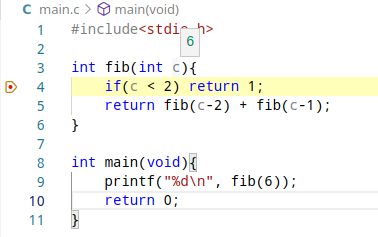
\includegraphics[height=.5\textheight]{vscode-dbg-decoration.png}
            \end{minipage}
            \hfill
            \begin{minipage}{.45\textwidth}
                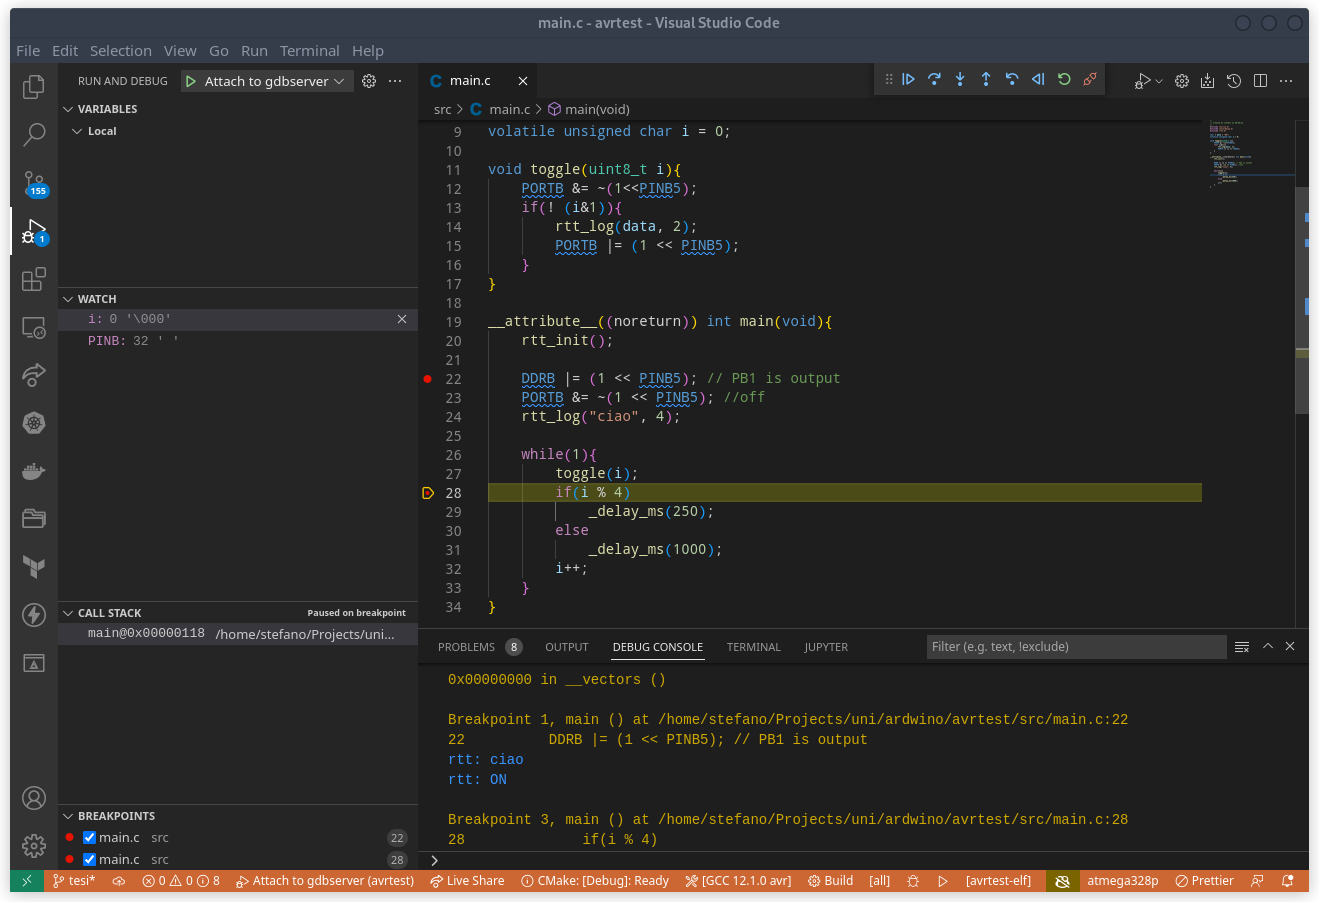
\includegraphics[height=.5\textheight]{vscode-dbg.png}
            \end{minipage}
        \end{figure}
    \end{frame}

    \begin{frame}
        \frametitle{Obiettivi}
        
        Sviluppo di un sistema che consenta quanto detto
        \begin{itemize}
            \item <1-> \textbf{Open Source}
            \item <2-> Debugging senza impiego di risorse
            \item <3-> \textit{Easy of Use}
            \item <4-> Monitor Debugging (\textit{Real Time Terminal})
        \end{itemize}
    \end{frame}

    \begin{frame}
        \frametitle{Stato dell'arte}
        La programmazione di dispositivi integrati viene effettuata tramite tre macro passaggi
        \begin{enumerate}
            \item<1-> Codifica $\rightarrow$
            {\footnotesize Il codice viene scritto dal programmatore e compilato in formato binario}
            \item<2-> Caricamento $\rightarrow$
            {\footnotesize Il programma viene scritto sulla memoria del controllore tramite l'uso di un programmatore}
            \item<3-> Esecuzione $\rightarrow$
            {\footnotesize Il controllore viene quindi avviato e il programma viene eseguito.}
        \end{enumerate}

        \begin{figure}
            \begin{tikzpicture}[scale=.8]
                \draw[fill=green!50] (0,0) rectangle (2,2) node[pos=.5] {\textit{host}};
                \draw[fill=yellow!50] (5,0.5) rectangle (8,1.5) node[pos=.5] {\textit{Programmer}};
                \draw[fill=blue!50] (11,0.5) rectangle (12.5,1.5) node[pos=.5] {\textit{target}};
                \node (0) at (1, -0.5) {1. Codifica};
                \node (0) at (6.5, -0.5) {2.Caricamento};
                \node (0) at (11.75, -0.5) {3. Esecuzione};
                \draw [stealth-stealth](2,1) -- (5,1) node[label={[font=\footnotesize]above:USB},pos=.5] {};
                \draw [stealth-stealth](8,1) -- (11,1) node[label={[font=\footnotesize]above:SPI/JTAG\cite{avr:appnote:isp}},pos=.5] {};
            \end{tikzpicture}
        \end{figure}
    \end{frame}
    \note{
        Il programmatore converte un protocollo complesso (USB/seriale) in comandi adatti alla programmazione dell'integrato su bus parallelo/spi
    }

    \begin{frame}
        \frametitle{Target}
    
        \begin{minipage}{.5\textwidth}
            \textbf{Arduino UNO R3}

            ATMega328P-PU\\{\footnotesize Processore a 8 bit, \SI{20}{MIPS}, \SI{20}{\mega\hertz}@\SI{5}{\volt}}\cite{avr:m328p}

            \begin{itemize}
                \item []<1-> \textbf{Pro}
                \begin{itemize}
                    \item <2-> Altamente diffuso e conosciuto\cite{site:arduino-uno-doc}
                    \item <3-> Community e open source
                    \item <4-> Debugger in hardware
                \end{itemize}
                \item []<4-> \textbf{Contro}
                \begin{itemize}
                    \item <5-> Architettura proprietaria
                    \item <6-> Protocollo di debugging non documentato\cite{site:dw-reverse-engeneering}
                \end{itemize}
            \end{itemize}            
        \end{minipage}
        \begin{minipage}{.48\textwidth}
            \begin{figure}
                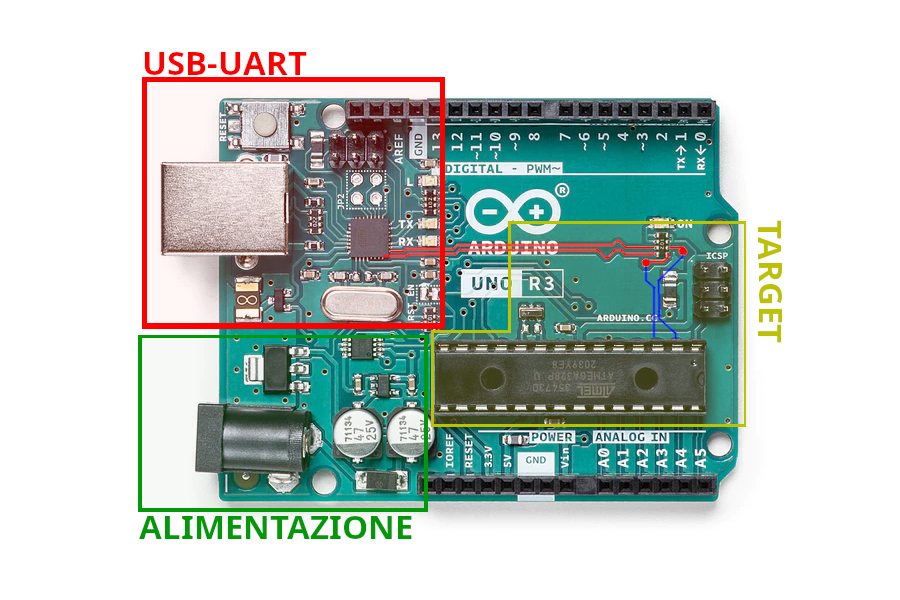
\includegraphics[width=\textwidth]{arduino-uno.png}
            \end{figure}    
        \end{minipage}
    \end{frame}


    \begin{frame}
        \frametitle{Architettura GDB}
    
        \begin{itemize}
            \item[] <1-> GDB è un software di \textit{debugging} multi-architettura open source
            \item[] <2-> Permette di lavorare su un processo remoto tramite l'architettura client-server
            \item[] <3-> Server GDB sul programmatore $\rightarrow$ {\footnotesize Converte i comandi del client nelle controparti del protocollo di debug}
        \end{itemize}
        \begin{figure}
            \begin{tikzpicture}
                \draw[fill=green!50] (0,0) rectangle (2,2) node[pos=.5] {Client};
                \draw[fill=yellow!50] (5,0.5) rectangle (7,1.5) node[pos=.5] {Server};
                \draw[fill=purple!50] (7,0.5) rectangle (8,1.5) node[pos=.5] {Conv};
                \draw[fill=red!50] (10.3,0.5) rectangle (11,1.5) node[pos=.5] {\small dW};
                \draw[fill=blue!50] (11,0.5) rectangle (12.5,1.5) node[pos=.5] {\textit{target}};

                \draw [stealth-stealth](2,1) -- (5,1) node[label={[font=\footnotesize]above:Protocollo GDB},pos=.5] {};
                \draw [stealth-stealth](8,1) -- (10.3,1) node[label={[font=\footnotesize]above:DebugWire\cite{site:dw-reverse-engeneering}},pos=.5] {};

                \draw (4.8, 0) rectangle (11.2, 2);
                \node (0) at (8, 2.5) {Ambito di sviluppo};
            \end{tikzpicture}
        \end{figure}
    \end{frame}
    \note{
        È possibile notare la similitudine con l'architettura host-programmatore-target
    }

    \begin{frame}
        \frametitle{Implementazione}
    
        \begin{figure}
            \begin{tikzpicture}[scale=.7]
                \node[inner sep=0pt] (arduino) at (0,0) {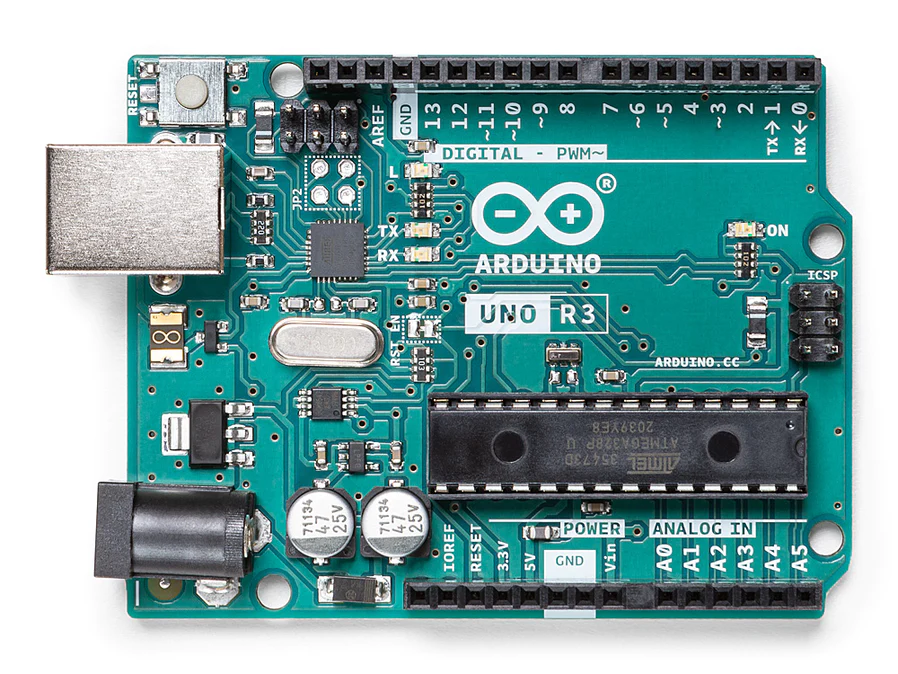
\includegraphics[width=.35\textwidth]{arduino-no-annotations.png}};

                \draw [fill=green!50] (-8, 0) rectangle (-6, 2) node [pos=.5] {Host};
                \draw [fill=yellow!50] (-1.1, 0.45) rectangle (-0.65, 0.88) node [pos=.5] {A};
                \draw [fill=blue!50] (2.75, -0.55) rectangle (-0.15, -1.15) node [pos=.5] {Target};

                \draw [semithick] (-6, 1) -- (-3.1, 1) node[pos=.5, label={above:USB}] {};
                \draw [color=yellow, thick] (-1.8, 1) -- (-1.45, 1) -- (-1.235, 0.665) -- (-1.1, 0.665);
                \draw [color=red, thick] (-0.65, 0.665) -- (2.3, 0.665) -- (2.5, 0.465) -- (2.5, -0.3) -- (2.7, -0.5);
            \end{tikzpicture}
        \end{figure}

        La scheda Arduino implementa la comunicazione \textit{target-host} mediante un controllore (ATMega16U2)\cite{git:arduinocore}\pause

        È stato sviluppato un server GDB e l'adattatore per debugWire sull'ATMega16U2 presente sulla scheda Arduino.
    \end{frame}

    

    \begin{frame}
        \frametitle{Circuito di Reset}

        \begin{minipage}{.5\textwidth}
            Il reset avviene all'asserzione della linea di reset\pause
        
            Due modi di effettuare il reset:
            \begin{itemize}
                \item L'utente preme il pulsante \texttt{RESET}
                \item Viene asserita la linea \texttt{DTR} (RS232)\cite{site:rs232}
            \end{itemize}
        \end{minipage}
        \begin{minipage}{.48\textwidth}
            \begin{figure}
                %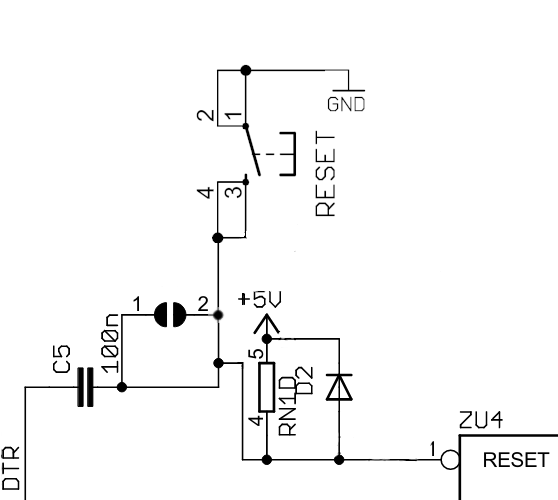
\includegraphics[width=\textwidth]{r3-rst-cap-pres-no-annotation.png}
                \begin{circuitikz}[scale=.8]
                    \draw (0, 0) node[label={[font=\footnotesize]above:\(\overline{\text{DTR}}\)}] {}
                    to[short, *-] (1, 0) [C=C5] to (2,0);
                    \draw (2,0) to[short, -*] (5, 0) node[label={[font=\footnotesize]above:\(\overline{\text{RST}}\)}] {};

                    \draw (3,0) to[short, *-] (3, 1)[R] to (3,2);
                    \draw (4,0) to[short, *-] (4, 1)[D] to (4,2);

                    \draw (3,0) to (3, -1) [nopb] to (3, -2);
                    \draw (3,-2) to (3, -3);

                    
                    \draw (3,2) to (3,2.5) to (3.5,2.5) to (3.5, 3);
                    \draw (4,2) to (4,2.5) to (3.5,2.5);
                    \draw (3,3) -- (4, 3) node[pos=.5, label=above:VCC] {};
                    \draw (2.5,-3) -- (3.5, -3) node[pos=.5, label=below:GND] {};

                \end{circuitikz}
            \end{figure}
        \end{minipage}
        
    \end{frame}
    
    \begin{frame}
        \frametitle{DebugWire}
    
        È il protocollo di debug di ATMega328P\pause

        È basato su protocollo fisico UART su linea open drain $\Rightarrow$ richiede una connessione diretta al pin di reset\pause

        Sostituisce la funzionalità di reset.
    \end{frame}

    \begin{frame}
        \frametitle{Modifiche Hardware}
        
        \noindent\begin{minipage}{.5\textwidth}
            Sono necessarie modifiche alla scheda Arduino UNO per permettere il corretto funzionamento del protocollo GDB
            \begin{itemize}
                \item <1-> È necessario collegare direttamente la linea di reset a un pin dell'adattatore
                \item <2-> È necessario isolare carichi resistivi sulla linea
                \item <3-> È necessario isolare il pulsante di reset
            \end{itemize}
        \end{minipage}
        \begin{minipage}{.48\textwidth}
            \begin{figure}
                %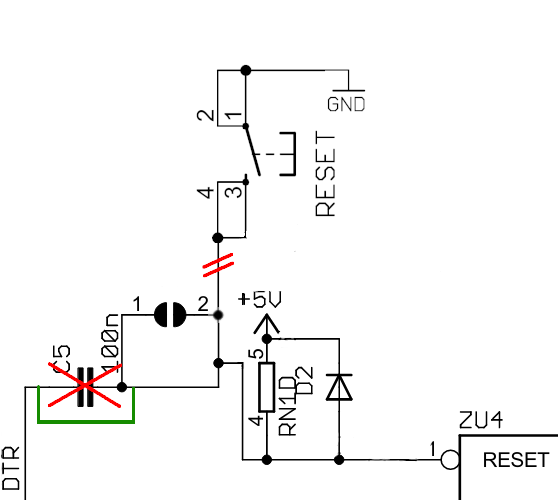
\includegraphics[width=\textwidth]{r3-rst-cap-pres.png}
                \begin{circuitikz}[scale=.8]
                    \draw (0, 0) node[label={[font=\footnotesize]above:\(\overline{\text{DTR}}\)}] {}
                    to[short, *-] (1, 0) [C=C5] to (2,0);
                    \draw (2,0) to[short, -*] (5, 0) node[label={[font=\footnotesize]above:\(\overline{\text{RST}}\)}] {};

                    \draw (3,0) to[short, *-] (3, 1)[R] to (3,2);
                    \draw (4,0) to[short, *-] (4, 1)[D] to (4,2);

                    \draw (3,0) to (3, -1) [nopb] to (3, -2);
                    \draw (3,-2) to (3, -3);

                    
                    \draw (3,2) to (3,2.5) to (3.5,2.5) to (3.5, 3);
                    \draw (4,2) to (4,2.5) to (3.5,2.5);
                    \draw (3,3) -- (4, 3) node[pos=.5, label=above:VCC] {};
                    \draw (2.5,-3) -- (3.5, -3) node[pos=.5, label=below:GND] {};

                    \draw [red] (1, -0.5) -- (2, 0.5);
                    \draw [red] (1, 0.5) -- (2, -0.5);

                    \draw [red] (2.75, -0.5) -- (3.25, -0.5);
                    \draw [red] (2.75, -0.7) -- (3.25, -0.7);

                    \draw [green, short, *-] (0.5, 0) to (0.5, -1) -- (2.5, -1) to[green, short, -*]  (2.5, 0);

                \end{circuitikz}
            \end{figure}
        \end{minipage}    
    \end{frame}
    
    \begin{frame}
        \frametitle{Server GDB}
        
        Sono state implementate funzionalità aggiuntive quali
        \begin{itemize}
            \item <1-> Programmazione della memoria flash tramite debugWire
            \item <2-> Monitor debugging (RTT)
        \end{itemize}
    
    \end{frame}

    \begin{frame}
        \frametitle{Real Time Terminal}
        \hspace*{-10mm}\begin{minipage}{.7\textwidth}
            \begin{itemize}
                \item[] Firmware target
                \begin{enumerate}
                    \item <1-> Scrittura del messaggio in un buffer in locazione nota
                    \item <2-> Impostazione del flag \texttt{AVAILABLE} (locazione sram nota)
                    \item <3-> \texttt{asm("break");}
                \end{enumerate}
                \item[] <4-> Server gdb alla ricezione di un break
                \begin{enumerate}
                    \setcounter{enumi}{3}
                    \item <4-> Lettura flag \texttt{AVAILABLE} dalla SRAM del target
                    \item <5-> Se vero
                    \begin{enumerate}
                        \item <5-> Lettura del buffer dalla SRAM
                        \item <5-> Invio del messaggio al client
                        \item <5-> Ripresa dell'esecuzione
                    \end{enumerate}
                    \item <6-> Se falso
                    \begin{enumerate}
                        \item <6-> Invio notifica di interruzione al client
                    \end{enumerate}
                \end{enumerate}
            \end{itemize}     
        \end{minipage}
        \begin{minipage}{.28\textwidth}
            \begin{figure}
                \begin{tikzpicture}[scale=.8, label distance=-2mm]

                    \draw (0,0) rectangle (2,2) node[pos=.5] {\textit{firmware}};
                    \draw (4,0) rectangle (5,0.2);
                    \draw (4,0.2) rectangle (5,0.4);
                    \draw (4,0.4) rectangle (5,1) node[pos=.5] {\tiny ...};
                    \draw (4,1) rectangle (5,1.4) node[pos=.5] {\tiny buffer};
                    \draw (4,1.4) rectangle (5,1.7) node[pos=.5] {\tiny avail};
                    \draw (4,1.7) rectangle (5,2)  node[pos=.5] {\tiny SRAM};
                    

                    \draw (0,3.5) rectangle (5,4.5) node[pos=.5] {\textit{Server}};

                    \draw (0,6) rectangle (5,7) node[pos=.5] {\textit{Client}};

                    \draw (-0.2,-0.5) rectangle (5.2,2.2) node[pos=.08] {\hspace*{5mm}\small\textit{Target}};


                    \draw[-stealth] (2,1.15) -- (4,1.15) node[pos=.25, label={above: \tiny 1}] {};
                    \draw[-stealth] (2,1.5) -- (4,1.5) node[pos=.25, label={above:\tiny 2}] {};
                    \draw[-stealth] (1,2) -- (1,3.5) node[pos=.5, label={right:\tiny 3}] {};
                    
                    \draw[-stealth] (2,3.5) -- (4,1.6) node[pos=.5, label={above:\tiny 4}] {};

                    \draw[-stealth] (1.5,3.5) -- (4,1.25) node[pos=.3, label={below:\tiny 5.1}] {};
                    \draw[-stealth] (1, 4.5) -- (1,6) node[pos=.5, label={left:\tiny 5.2}] {};
                    \draw[-stealth] (0.5,3.5) -- (0.5,2) node[pos=.5, label={left:\tiny 5.3}] {};

                    \draw[-stealth] (1.5, 4.5) -- (1.5,6) node[pos=.5, label={right:\tiny 6.1}] {};
                \end{tikzpicture}
            \end{figure}
        \end{minipage}
    \end{frame}

    \begin{frame}
        \frametitle{Difficoltà}
    
        Lo sviluppo del sistema ha incontrato difficoltà nei seguenti ambiti
        \begin{itemize}
            \item Comunicazione USB\\{\footnotesize Comprensione del protocollo USB-CDC e della libreria che lo implementa (LUFA)}
            \item Implementazione della comunicazione fisica
            \item Dimensione del firmware finale (\SI{15}{KiB})
        \end{itemize}
    
    \end{frame}
    
    \begin{frame}
        \frametitle{Conclusioni e sviluppi futuri}
    
        \begin{itemize}
            \item <1-> Adattamento di un'IDE al sistema
            \begin{itemize}
                \item <2-> Integrazione di GDB
                \item <3-> Sviluppo di un sistema di compilazione
            \end{itemize}
            \item <4-> Progetto open source
            \item <5-> Sarà possibile sviluppare nuove versioni sfruttando le funzionalità offerte da questa versione.
        \end{itemize}
    

    \end{frame}

    \appendix
    \begin{frame}
        tank u bitches
    \end{frame}
    
    %\begin{frame}
    %    \frametitle{Implementazione \hfill 1}
    %
    %    \begin{figure}
    %        \begin{tikzpicture}[scale=0.80]
    %            \draw[fill=green!50] (0,3) rectangle (4,4) node[pos=.5] {GDB}; %GDB
    %            \draw[fill=yellow!50] (0,2) rectangle (4,3) node[pos=.5] {GDB proto}; %gdb_proto
    %            \draw[fill=red!50] (0,1) rectangle (4,2) node[pos=.5] {CDC}; %cdc
    %            \draw[fill=blue!50] (0,0) rectangle (4,1) node[pos=.5] {USB PHY}; %usb_phy
    %            
    %            \draw[fill=purple!50,purple!50,text=black] (5,3) rectangle (9,4) node[pos=.5] {GDB server}; %GDB_SERVER
    %            \draw[fill=purple!50,purple!50] (7.5,2) rectangle (9,3); 
    %            \draw (5,3) -- (5,4) -- (9,4) -- (9,2);
    %            \draw[fill=yellow] (7.75,2) rectangle (8.75,2.5) node[pos=.5] {RTT}; %RTT
    %    
    %            \draw[fill=yellow!50] (5,2) rectangle (7.5,3) node[pos=.5] {GDB proto}; %gdb_proto
    %            \draw[fill=red!50] (5,1) rectangle (7.5,2) node[pos=.5] {CDC}; %cdc
    %            \draw[fill=blue!50] (5,0) rectangle (7.5,1) node[pos=.5] {USB PHY}; %usb_phy
    %            \draw[fill=gray!50] (7.5,1) rectangle (9,2) node[pos=.5] {dW}; %dw
    %            \draw[fill=orange!50] (7.5,0) rectangle (9,1) node[pos=.5] {UART}; %uart
    %    
    %            \draw[fill=cyan!50] (10,2) rectangle (14,3) node[pos=.5] {Process}; %AVR
    %            \draw[fill=yellow] (12.75,2) rectangle (13.75,2.5) node[pos=.5] {RTT}; %RTT
    %            \draw[fill=gray!50] (10,1) rectangle (14,2) node[pos=.5] {dW}; %dw
    %            \draw[fill=orange!50] (10,0) rectangle (14,1) node[pos=.5] {UART (O.D.)}; %UART
    %    
    %            \draw[black, thick] (2, 0) -- (2, -0.5) -- (6.25, -0.5) -- (6.25, 0);
    %            \draw[black, thick] (8.5,0) -- (8.5, -0.5) -- (12, -0.5) -- (12, 0);
    %    
    %            \node (5) at (2, 4.5) {Host};
    %            \node (5) at (7, 4.5) {Adapter};
    %            \node (5) at (12, 4.5) {Tagret (AVR)};
    %        \end{tikzpicture}
    %    \end{figure}
    %\end{frame}
%
    %\begin{frame}
    %    \frametitle{Implementazione \hfill 2}
    %
    %    \begin{figure}
    %        \begin{tikzpicture}
    %            \node[inner sep=0pt] (arduino) at (0,0) {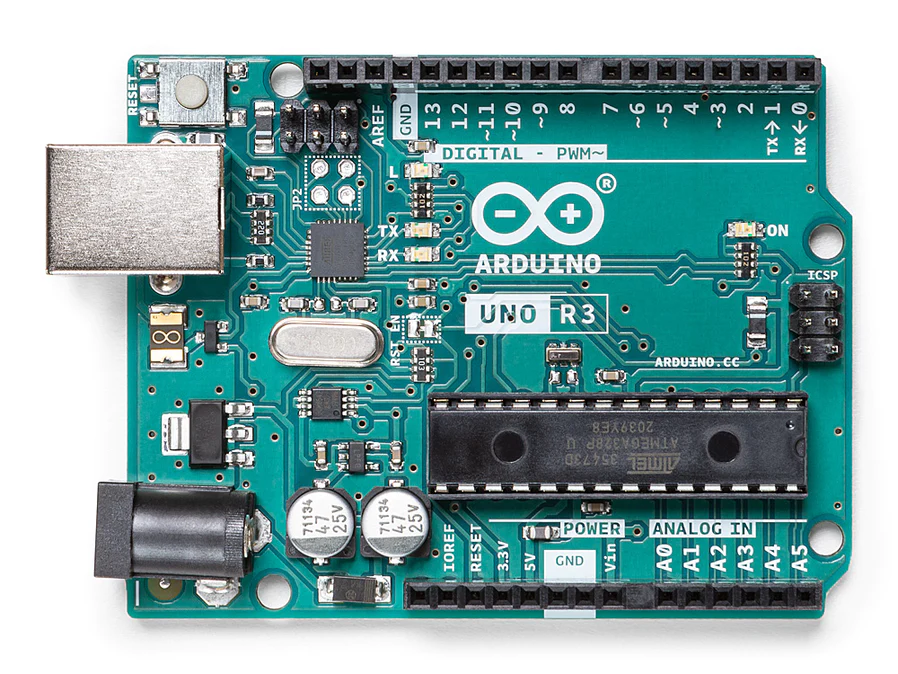
\includegraphics[width=.5\textwidth]{arduino-no-annotations.png}};
%
    %            \draw [fill=green!50] (-8, 0) rectangle (-6, 2) node [pos=.5] {Host};
    %            \draw [fill=yellow!50] (-1.1, 0.45) rectangle (-0.65, 0.88) node [pos=.5] {A};
    %            \draw [fill=blue!50] (2.75, -0.55) rectangle (-0.15, -1.15) node [pos=.5] {Target};
%
    %            \draw [semithick] (-6, 1) -- (-3.1, 1);
    %            \draw [color=yellow, thick] (-1.8, 1) -- (-1.45, 1) -- (-1.235, 0.665) -- (-1.1, 0.665);
    %            \draw [color=red, thick] (-0.65, 0.665) -- (2.3, 0.665) -- (2.5, 0.465) -- (2.5, -0.3) -- (2.7, -0.5);
    %        \end{tikzpicture}
    %    \end{figure}
    %\end{frame}
%
    %\begin{frame}
    %    \frametitle{Modifiche hardware}
    %    \begin{minipage}{.55\textwidth}
    %        Al fine di rendere la scheda compatibile con il protocollo debug wire:
    %        \begin{itemize}
    %            \item <1-> È stato rimosso il condensatore che isolava la connessione tra il pin dell'integrato adattatore e controllore target
    %            \item <2->  Sono state isolate alcune resistenza di pull-down
    %            \item <3->  È stato isolato il pulsante di reset
    %        \end{itemize}
    %    \end{minipage}
    %    \begin{minipage}{.44\textwidth}
    %        \begin{figure}
    %            \hfill
    %            \begin{minipage}{.45\textwidth}
    %                \subfloat[][]{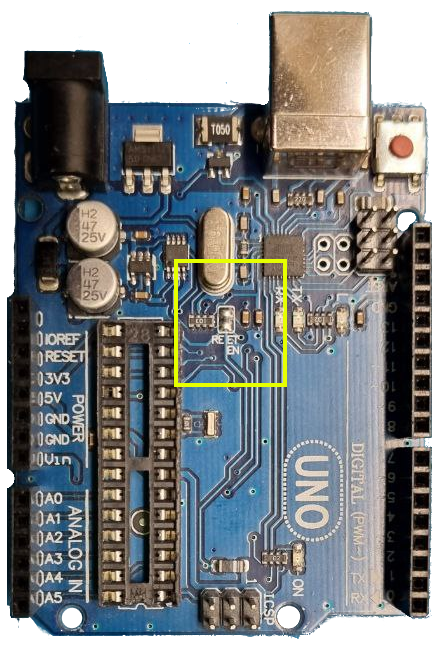
\includegraphics[width=.9\textwidth]{cap_begin.png}}
    %            \end{minipage}
    %            \begin{minipage}{.45\textwidth}
    %                \subfloat[][]{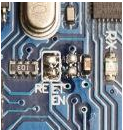
\includegraphics[width=.5\textwidth]{cap_removed.png}} \\
    %                \subfloat[][]{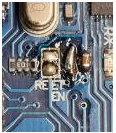
\includegraphics[width=.5\textwidth]{cap_shorted.png}}
    %            \end{minipage}
    %            \hfill
    %        \end{figure}
    %    \end{minipage}
    %
    %\end{frame}
%
    %\begin{frame}
    %    \frametitle{Risultati}
    %    
    %    \begin{figure}
    %        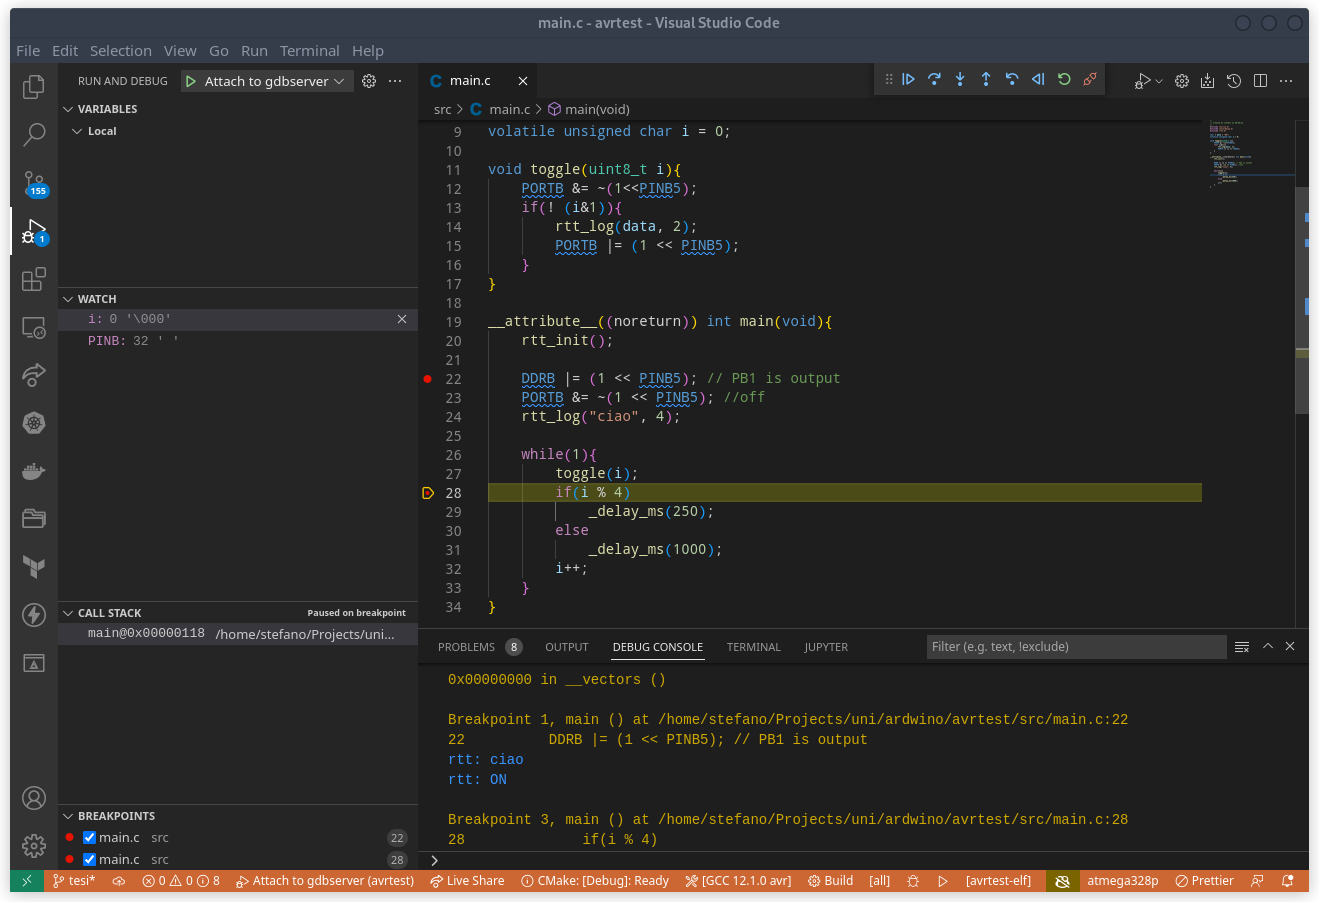
\includegraphics[height=.7\textheight]{vscode-dbg.png}
    %    \end{figure}
    %
    %\end{frame}
%
    \begin{frame}[allowframebreaks]
        \frametitle{Bibliografia e Sitografia}
        \printbibliography[heading=none]%
    \end{frame}

\end{document}
